\documentclass[conference]{IEEEtran}
\IEEEoverridecommandlockouts

% ---------------------------------------------------------
% PAQUETES
% ---------------------------------------------------------
\usepackage[utf8]{inputenc}
\usepackage[spanish,es-tabla]{babel}
\usepackage{amsmath,amssymb}
\usepackage{graphicx}
\usepackage{booktabs}
\usepackage{multirow}
\usepackage{array}
\usepackage{longtable}
\usepackage{hyperref}
\usepackage{float}
\usepackage{xcolor}
\usepackage{enumitem}

\hypersetup{
    colorlinks=true,
    linkcolor=black,
    citecolor=black,
    urlcolor=blue
}

% ---------------------------------------------------------
% INFORMACIÓN DEL DOCUMENTO
% ---------------------------------------------------------

\title{Comportamiento Adaptativo y Toma de Decisiones en Agentes Ecológicos mediante Aprendizaje por Refuerzo: Revisión y Evaluación Experimental}

\author{
\IEEEauthorblockN{Axel López Vega}
\and
\IEEEauthorblockN{Kevin Núñez Camacho}
\and
\IEEEauthorblockN{Felipe Murillo}
}

% ---------------------------------------------------------
% DOCUMENTO
% ---------------------------------------------------------

\begin{document}

\maketitle

% ---------------------------------------------------------
% RESUMEN
% ---------------------------------------------------------

\begin{abstract}

El estudio computacional del comportamiento animal requiere representar
individuos capaces de responder ante cambios en el ambiente, disponibilidad
de recursos, amenazas y relaciones con otros individuos. Los Modelos
Basados en Agentes (ABM) permiten representar estos sistemas mediante
entidades autónomas, mientras que el Aprendizaje por Refuerzo (RL) permite
estudiar cómo dichas entidades pueden aprender estrategias de decisión a
partir de su interacción con el entorno.

Este trabajo presenta una revisión de literatura de 21 trabajos
relacionados con aprendizaje por refuerzo, modelado basado en agentes,
teoría de forrajeo, sistemas multiagente y comportamiento emergente, y
complementa dicha revisión con el diseño y la evaluación experimental de un
simulador 2D de un ecosistema con herbívoros y carnívoros. El problema se
formula como un proceso de decisión de Markov con observación local, acciones
discretas y recompensas orientadas a la supervivencia y al equilibrio
ecológico.

Los trabajos revisados permiten identificar como elementos recurrentes la
incorporación de variables fisiológicas, información espacial, percepción
parcial, memoria y diferentes estructuras de recompensa. Sobre esta base se
entrena una política REINFORCE y se compara con políticas aleatoria y
heurística mediante cinco semillas independientes. También se reporta un
análisis de sensibilidad de la tasa de aprendizaje con tres configuraciones y
tres semillas por configuración, incluyendo curvas de aprendizaje, dispersión
y métricas de éxito, recompensa y longitud de episodio.

\end{abstract}

% ---------------------------------------------------------
% 1. INTRODUCCIÓN
% ---------------------------------------------------------

\section{Introducción}

Los ecosistemas pueden entenderse como sistemas dinámicos en los que
múltiples organismos interactúan entre sí y con un ambiente que cambia
constantemente. Las decisiones de cada individuo pueden estar
condicionadas por factores internos, como su nivel energético o estado
fisiológico, y por factores externos, como la disponibilidad de alimento,
la presencia de depredadores, la distribución de recursos y la presencia
de otros individuos. Debido a esta combinación de factores, representar
computacionalmente el comportamiento ecológico constituye un problema que
requiere considerar tanto las características individuales como las
interacciones que ocurren dentro del sistema.

Los Modelos Basados en Agentes (ABM) constituyen una alternativa para
representar estos sistemas mediante individuos autónomos. En un ABM, cada
agente posee un estado y puede ejecutar acciones que modifican su propia
situación o afectan al entorno y a otros agentes. Esta característica ha
permitido utilizar este tipo de modelos para estudiar fenómenos
ecológicos en los que los patrones observados a nivel colectivo son
consecuencia de las decisiones individuales.

Sin embargo, una dificultad de los modelos tradicionales consiste en la
definición de las reglas que controlan el comportamiento de los agentes.
Cuando las decisiones se representan mediante reglas predeterminadas, el
diseñador debe especificar de antemano cómo debe responder el agente ante
las diferentes situaciones posibles. Este enfoque puede resultar
limitante cuando se pretende estudiar escenarios que no fueron
contemplados durante la construcción del modelo.

El Aprendizaje por Refuerzo (RL) proporciona una alternativa basada en el
aprendizaje mediante interacción con el entorno. En lugar de establecer
directamente todas las decisiones mediante reglas, un agente puede
aprender una política que determine qué acción ejecutar a partir del
estado que observa y de las recompensas obtenidas. Esta característica
permite estudiar si determinadas estrategias pueden surgir como
consecuencia del proceso de aprendizaje.

En los trabajos analizados se encuentran aplicaciones de este enfoque a
problemas como el forrajeo, la selección de recursos, la respuesta ante
depredadores, la adaptación a la escasez y la coordinación entre
individuos. Algunos trabajos incorporan además mecanismos de memoria,
variables fisiológicas y observabilidad parcial, buscando representar de
manera más cercana las condiciones bajo las cuales los organismos toman
decisiones.

Un aspecto especialmente relevante para este tipo de modelos es que el
comportamiento aprendido depende de la forma en que se representa el
estado del agente y de la función de recompensa utilizada. Una
representación demasiado limitada puede impedir que el agente disponga
de la información necesaria para tomar una decisión adecuada. Por otro
lado, una recompensa mal definida puede incentivar estrategias que
maximicen la recompensa matemática sin representar el comportamiento
ecológico que se pretendía estudiar.

Este último problema se relaciona con el concepto de
\textit{reward misspecification}, mediante el cual una función de
recompensa no representa de forma adecuada el objetivo que se desea
alcanzar. En sistemas ecológicos, este problema adquiere especial
importancia debido a que conceptos como supervivencia, bienestar,
eficiencia energética o cooperación pueden depender de múltiples
variables y no necesariamente pueden representarse mediante una única
señal de recompensa.

A partir de esta problemática, el presente survey analiza trabajos que
utilizan aprendizaje por refuerzo y modelos basados en agentes para
representar comportamientos individuales y colectivos en ambientes
ecológicos. El análisis se concentra principalmente en la relación entre
las condiciones ambientales, la representación del estado, las
estructuras de recompensa y los comportamientos que emergen durante el
aprendizaje.

La revisión se orienta mediante las siguientes preguntas de
investigación:

\begin{itemize}

    \item \textbf{PI1:} ¿Cómo emergen los comportamientos adaptativos y
    las estrategias de supervivencia colectiva o individual en los
    agentes simulados ante escenarios de estrés ambiental o escasez de
    recursos?

    \item \textbf{PI2:} ¿Cuáles son las variables de estado
    (sensoriales e internas) y las estructuras de funciones de recompensa
    más efectivas para modelar la toma de decisiones ecológicas sin
    generar sesgos o conductas no deseadas
    (\textit{reward misspecification})?

\end{itemize}

El objetivo de la revisión no consiste únicamente en describir los
trabajos seleccionados, sino en identificar patrones comunes entre ellos,
comparar las estrategias utilizadas y determinar qué elementos del diseño
de los agentes parecen ser relevantes para producir comportamientos
adaptativos y ecológicamente plausibles.

% ---------------------------------------------------------
% 2. METODOLOGÍA DE LA REVISIÓN
% ---------------------------------------------------------

\section{Metodología de la revisión}

El presente trabajo corresponde a una revisión de literatura centrada en
el uso de técnicas de aprendizaje por refuerzo y modelos basados en
agentes para representar procesos de decisión y comportamiento ecológico.
El conjunto de análisis está compuesto por 21 trabajos seleccionados por
su relación con las preguntas de investigación planteadas.

Los trabajos abarcan diferentes perspectivas. Algunos estudian
directamente el comportamiento de agentes individuales durante tareas de
forrajeo, mientras que otros analizan sistemas multiagente, coordinación,
competencia, cooperación y formación de estructuras colectivas. También
se incluyen trabajos relacionados con memoria, modelos del mundo,
dinámicas depredador-presa, homeostasis y diseño de entornos de
simulación.

Debido a esta diversidad, la comparación no se realiza únicamente a
partir del algoritmo empleado. En su lugar, los trabajos se analizan
considerando los elementos que determinan el comportamiento del agente y
la manera en que este comportamiento es evaluado.

\subsection{Dimensiones de análisis}

Para realizar la comparación de los trabajos se establecieron cuatro
dimensiones principales:

\begin{enumerate}

    \item \textbf{Representación del estado:} información disponible para
    el agente, incluyendo variables internas, información ambiental,
    información espacial, vecinos y memoria.

    \item \textbf{Función de recompensa:} mecanismo utilizado para
    incentivar determinadas acciones o resultados durante el proceso de
    aprendizaje.

    \item \textbf{Entorno e interacción:} características del ambiente de
    simulación, disponibilidad de recursos, amenazas, número de agentes
    y nivel de observabilidad.

    \item \textbf{Comportamiento y evaluación:} estrategias individuales
    o colectivas observadas y métricas utilizadas para determinar si el
    comportamiento aprendido cumple con el objetivo planteado.

\end{enumerate}

Estas dimensiones permiten comparar estudios que emplean algoritmos
diferentes pero que presentan problemas ecológicos similares. Por
ejemplo, un trabajo puede utilizar aprendizaje por refuerzo profundo para
estudiar forrajeo individual, mientras otro puede utilizar aprendizaje
multiagente para estudiar coordinación. Aunque los algoritmos sean
distintos, ambos pueden proporcionar evidencia sobre la influencia de la
representación del estado o de la función de recompensa en el
comportamiento obtenido.

\subsection{Clasificación temática}

A partir de las dimensiones anteriores, los trabajos se organizarán en
cuatro áreas temáticas principales:

\begin{enumerate}

    \item \textbf{Forrajeo y adaptación ante escasez de recursos.}
    Incluye trabajos relacionados con búsqueda de alimento, explotación
    de recursos, exploración, agotamiento de parches y supervivencia.

    \item \textbf{Estado, percepción y memoria.}
    Comprende investigaciones que analizan variables fisiológicas,
    información espacial, observabilidad parcial, memoria y
    representaciones internas.

    \item \textbf{Recompensas y homeostasis.}
    Incluye trabajos centrados en funciones de recompensa, objetivos
    individuales o colectivos, homeostasis y problemas derivados de una
    especificación incorrecta de las recompensas.

    \item \textbf{Comportamiento colectivo y sistemas multiagente.}
    Comprende estudios sobre cooperación, competencia, coordinación,
    agrupamiento, formación de bandadas y otros comportamientos
    colectivos.

\end{enumerate}

Esta clasificación se utilizará posteriormente para organizar la
discusión de los resultados. Un mismo trabajo puede aportar evidencia a
más de una categoría, debido a que la representación del estado, la
recompensa y la interacción entre agentes se encuentran estrechamente
relacionadas.

\subsection{Criterios de comparación}

Además de la clasificación temática, cada trabajo será comparado
considerando las siguientes características:

\begin{table}[H]
\centering
\caption{Dimensiones utilizadas para el análisis comparativo}
\label{tab:dimensiones}
\small
\begin{tabular}{p{3.5cm} p{4.5cm}}
\toprule
\textbf{Dimensión} & \textbf{Aspecto considerado} \\
\midrule

Algoritmo &
Técnica de aprendizaje por refuerzo utilizada y paradigma de
entrenamiento. \\

Estado &
Variables internas, ambientales, espaciales, sociales y temporales
disponibles para el agente. \\

Observabilidad &
Información completa o parcial disponible durante la toma de
decisiones. \\

Recompensa &
Tipo de recompensa, objetivo incentivado y nivel de especificidad. \\

Entorno &
Características del ambiente, distribución de recursos, amenazas y
dinámica ambiental. \\

Interacción &
Número de agentes y presencia de cooperación, competencia o
coordinación. \\

Comportamiento &
Estrategias individuales o colectivas observadas durante la simulación. \\

Evaluación &
Métricas utilizadas para evaluar aprendizaje, supervivencia y
comportamiento emergente. \\

\bottomrule
\end{tabular}
\end{table}

% ---------------------------------------------------------
% 3. FUNDAMENTOS CONCEPTUALES
% ---------------------------------------------------------

\section{Fundamentos conceptuales}

Esta sección presenta los conceptos necesarios para interpretar los
resultados de la revisión. Debido a que el objetivo principal del trabajo
es analizar la literatura y no desarrollar una introducción extensa a
cada técnica, los conceptos se presentan únicamente desde la perspectiva
de su utilización en sistemas ecológicos.

\subsection{Modelos Basados en Agentes}

Los Modelos Basados en Agentes permiten representar sistemas complejos
mediante individuos autónomos que interactúan entre sí y con un entorno.
Cada agente puede poseer un conjunto de variables que describe su estado,
un conjunto de acciones disponibles y mecanismos para modificar su
comportamiento.

En un contexto ecológico, un agente puede representar un organismo que
posee características como posición, energía, nivel de hambre,
información sensorial y experiencias anteriores. El entorno puede incluir
recursos, obstáculos, depredadores y otros individuos.

Una característica importante de los ABM es que permiten estudiar cómo
las decisiones individuales pueden producir patrones a nivel colectivo.
Por esta razón, resultan adecuados para investigar fenómenos como
agrupamiento, cooperación, competencia o formación de bandadas.

Sin embargo, en un ABM tradicional las decisiones pueden depender de
reglas diseñadas manualmente. El aprendizaje por refuerzo permite
modificar este enfoque al permitir que el agente aprenda una política de
decisión mediante la interacción con el entorno.

\subsection{Aprendizaje por Refuerzo}

El Aprendizaje por Refuerzo estudia el proceso mediante el cual un agente
aprende a seleccionar acciones a partir de su interacción con un entorno.
En una formulación simplificada, el proceso puede representarse como:

\begin{equation}
s_t \rightarrow a_t \rightarrow r_t \rightarrow s_{t+1}
\end{equation}

donde $s_t$ representa el estado del agente en el instante $t$, $a_t$
representa la acción seleccionada, $r_t$ corresponde a la recompensa
obtenida y $s_{t+1}$ representa el nuevo estado.

El objetivo del agente consiste en aprender una política que permita
obtener recompensas acumuladas elevadas. En aplicaciones ecológicas, las
acciones pueden representar desplazarse, consumir alimento, descansar,
huir de un depredador o interactuar con otros individuos.

La importancia de este enfoque para la presente revisión radica en que
permite estudiar qué estrategias aparecen cuando el agente debe aprender
a partir de las consecuencias de sus propias acciones.

\subsection{Aprendizaje por Refuerzo Profundo}

El Aprendizaje por Refuerzo Profundo (DRL) combina el aprendizaje por
refuerzo con redes neuronales utilizadas para aproximar funciones de
valor, políticas o representaciones del estado.

Su utilización resulta relevante cuando el espacio de estados presenta
una cantidad elevada de variables o cuando las relaciones entre las
variables no pueden representarse fácilmente mediante estructuras
tabulares.

Dentro de los trabajos revisados, el DRL aparece asociado a problemas
como forrajeo, conservación, percepción visual y modelado de ecosistemas.
Sin embargo, el uso de una red neuronal por sí mismo no garantiza la
aparición de un comportamiento ecológicamente válido. La información
proporcionada al agente y la función de recompensa continúan siendo
elementos fundamentales.

\subsection{Observabilidad parcial y memoria}

En un ambiente ecológico, un agente normalmente no tiene acceso a toda la
información existente en el entorno. Su percepción puede estar limitada
por la distancia, el campo de visión, obstáculos o las capacidades
sensoriales del organismo representado.

Esta situación puede formularse mediante un Proceso de Decisión de Markov
Parcialmente Observable (POMDP), donde el agente debe tomar decisiones
utilizando únicamente una observación parcial del estado real del
entorno.

La observabilidad parcial hace que la memoria pueda adquirir un papel
importante. Un agente puede utilizar información de experiencias
anteriores para complementar su percepción actual. Esta información puede
corresponder a la ubicación de recursos, el tiempo desde una visita
anterior, la calidad de una zona o experiencias relacionadas con una
amenaza.

Por lo tanto, la memoria puede considerarse un componente de la
representación del estado cuando la información necesaria para tomar una
decisión no está disponible directamente en el momento actual.

\subsection{Aprendizaje por Refuerzo Multi-Agente}

Cuando varios agentes aprenden e interactúan simultáneamente, el problema
se extiende al Aprendizaje por Refuerzo Multi-Agente (MARL). En este caso,
las acciones de un agente pueden modificar el entorno observado por los
demás.

En un escenario ecológico, por ejemplo, varios individuos pueden consumir
el mismo recurso, competir por una fuente de alimento o beneficiarse de
permanecer juntos. Como consecuencia, el aprendizaje de cada agente puede
afectar el proceso de aprendizaje de los demás.

Esta interacción introduce problemas como la no-estacionariedad,
coordinación y asignación de crédito (\textit{credit assignment}). Al
mismo tiempo, permite estudiar cómo pueden surgir comportamientos
colectivos a partir de decisiones individuales.

\subsection{Comportamiento emergente}

Para efectos de esta revisión, se considera comportamiento emergente
aquel patrón observable que resulta de la interacción entre los agentes,
el entorno y las reglas de aprendizaje, sin necesidad de definir
explícitamente dicho patrón como una regla de comportamiento.

Entre los comportamientos analizados en los trabajos se encuentran la
cooperación, competencia, coordinación, formación de grupos, evasión
colectiva y adaptación ante cambios en la disponibilidad de recursos.

La distinción entre comportamiento programado y comportamiento emergente
es importante para esta revisión. Si una función de recompensa obliga
directamente al agente a producir un patrón determinado, observar dicho
patrón no necesariamente demuestra que haya surgido como consecuencia de
la interacción con el entorno.

Por esta razón, los trabajos se analizarán no solamente considerando qué
comportamiento aparece, sino también las condiciones bajo las cuales
aparece y la forma en que los autores determinan que dicho comportamiento
es realmente emergente.

% ---------------------------------------------------------
% 4. Análisis temático de la literatura
% ---------------------------------------------------------

\section{Análisis de la literatura}

Como paso previo al desglose conceptual, y para facilitar la contrastación 
metodológica de los distintos enfoques, la 
\textbf{Tabla \ref{tab:comparativa_completa}} (ubicada en esta sección) sintetiza los 
trabajos más representativos de la revisión. Esta matriz cruza las 
técnicas algorítmicas, los entornos de simulación (datasets/Gridworlds), 
las métricas principales y, de manera crítica, las limitaciones 
identificadas en cada estudio. A partir del mapeo expuesto en la tabla, 
la literatura se analiza a través de las siguientes cuatro dimensiones 
fundamentales:

\subsection{Forrajeo y adaptación ante la escasez de recursos}
La literatura demuestra que el forrajeo óptimo ante la escasez no depende de 
reglas fijas, sino de la capacidad de anticipación del agente. Los agentes que 
construyen representaciones internas o ''modelos del mundo'' logran planificar 
trayectorias de forrajeo óptimas ante recursos heterogéneos, convergiendo a 
estrategias de la teoría clásica del Teorema del Valor Marginal sin requerir 
memorias tabulares rígidas. Asimismo, el agotamiento gradual de los recursos 
actúa como una fuente crucial de información; las aves aprenden la calidad 
inicial del parche basándose en el patrón de espaciado temporal entre bocados, 
optimizando su supervivencia mediante reglas de temporización en entornos 
variables. Además, los algoritmos de aprendizaje sin modelo (model-free) han 
demostrado descubrir estrategias autónomas ante situaciones críticas y puntos 
de inflexión ecológica, superando las reglas empíricas humanas frente a 
perturbaciones ambientales.

\subsection{Representación del estado, percepción y memoria}
Una representación de estado efectiva requiere combinar la percepción espacial 
con variables fisiológicas. La inclusión de señales de interocepción, como 
el nivel de saciedad, permite a los agentes adaptar su velocidad y realizar 
pausas voluntarias para conservar energía \cite{Paper1}. En entornos de 
escasez extrema, incorporar mecanismos de memoria episódica biológica resulta 
vital para que el agente recuerde qué, dónde y cuándo almacenó comida, 
evitando visitar celdas recién agotadas. El estado también suele estructurarse 
combinando variables internas de salud con información de una vecindad espacial
limitada ($3 x 3$) y señales de distancia a los recursos \cite{Paper2}. 
Para garantizar el realismo de estas simulaciones, los modelos deben basarse 
en resoluciones espaciales precisas que capturen la dinámica de la vegetación 
y el agua, elementos fundamentales para determinar la idoneidad del hábitat.

\subsection{Funciones de recompensa y homeostasis}
El diseño de las recompensas enfrenta el riesgo de generar conductas sesgadas 
(reward misspecification), donde el agente aprende atajos matemáticos en lugar 
de estrategias ecológicas. Para evitar recompensas dispersas, se proponen 
funciones de recompensa homeostáticas cuadráticas que incentivan mantener 
niveles internos de energía e hidratación equilibrados \cite{Paper2}. Estas 
funciones no lineales penalizan cuadráticamente tanto la deficiencia como la 
sobresaturación, obligando a la IA a buscar un equilibrio biológico en lugar 
de maximizar el consumo infinitamente. Adicionalmente, el estado interno debe 
interactuar con las amenazas del entorno; la ponderación de la recompensa 
mediante penalizaciones por riesgo de depredación permite modelar el conflicto 
biológico entre el hambre y el miedo. En simulaciones multiagente con escasez, 
las recompensas diseñadas a mano suelen fallar, haciendo necesaria la 
integración de redes predictoras (MARP) que evalúen el éxito a nivel 
poblacional en lugar del beneficio individual.

\subsection{Comportamiento colectivo y sistemas multiagente}
En entornos multiagente, el comportamiento emergente surge sin necesidad de 
programar reglas rígidas. En cuadrículas 2D acotadas, agentes perseguidores 
pueden desarrollar hasta 21 patrones de coordinación táctica excluyendo 
deliberadamente las recompensas densas por distancia y utilizando únicamente 
recompensas de resultado. La formación de bandadas con alto orden polar emerge 
de manera natural al aplicar funciones de costo local que penalizan tanto la 
dispersión excesiva como el hacinamiento entre individuos. Incluso en 
escenarios donde los individuos son egoístas y carecen de incentivos 
explícitos para cooperar, la agrupación (swarming) surge como estrategia 
adaptativa para compensar la observabilidad parcial del entorno. Sin embargo, 
la literatura advierte que un alto desempeño en términos de recompensa media 
no siempre implica cooperación biológica real, por lo que es necesario 
analizar estadísticamente las trayectorias para validar si la colaboración es 
causal o una ilusión estadística.

\subsection{Comparación de estrategias de modelado}

La comparación de los trabajos muestra que la representación del estado
constituye uno de los principales factores que diferencian los enfoques
revisados. Los modelos más simples utilizan principalmente información
espacial o distancia hacia recursos y otros agentes, mientras que los
modelos orientados a representar procesos ecológicos más complejos
incorporan variables internas como energía, hambre, hidratación o
saciedad.

También se observa una diferencia entre los modelos que utilizan
información directamente observable y aquellos que incorporan memoria o
representaciones internas. En ambientes donde los recursos cambian o
presentan una distribución temporal, la memoria permite utilizar
información obtenida en interacciones anteriores. De manera similar, la
observabilidad parcial obliga al agente a tomar decisiones sin disponer
del estado completo del ambiente.

En cuanto a las funciones de recompensa, los trabajos revisados
presentan desde recompensas simples asociadas con la obtención de
recursos hasta estructuras que consideran homeostasis, supervivencia,
riesgo y objetivos colectivos. Esta diferencia resulta especialmente
importante debido a que una recompensa demasiado específica puede
restringir el comportamiento del agente, mientras que una recompensa
demasiado general puede permitir estrategias que maximicen la señal
numérica sin representar adecuadamente el objetivo ecológico.

En los sistemas multiagente, esta situación se vuelve más compleja debido
a que el comportamiento de un agente puede modificar las condiciones
experimentadas por los demás. Por ello, algunos estudios utilizan
recompensas individuales, mientras que otros incorporan objetivos
compartidos o multiobjetivo. Los resultados revisados sugieren que la
cooperación y la coordinación no necesariamente deben programarse de
forma explícita, pero su aparición debe evaluarse cuidadosamente para
distinguir entre un comportamiento verdaderamente emergente y uno
producido directamente por el diseño de la recompensa.

\section{Síntesis de los hallazgos}

La literatura revisada permite observar que el comportamiento adaptativo
de los agentes no depende exclusivamente del algoritmo de aprendizaje
utilizado. La interacción entre la representación del estado, la función
de recompensa y las características del entorno tiene un papel
fundamental en las estrategias obtenidas.

En escenarios de escasez de recursos, los agentes pueden modificar sus
estrategias de exploración y explotación, utilizar información obtenida
de experiencias anteriores y responder a cambios en la disponibilidad de
recursos. Cuando además se incorporan múltiples agentes, estas decisiones
individuales pueden generar patrones colectivos como agrupamiento,
coordinación, cooperación o competencia.

De manera general, los estudios también muestran que incrementar la
complejidad del modelo no garantiza un comportamiento más realista. La
incorporación de variables adicionales debe responder a las capacidades
que se desean representar y a la información que tendría disponible el
organismo modelado. De forma similar, una función de recompensa más
compleja no necesariamente produce mejores resultados si introduce
incentivos contradictorios o comportamientos no deseados.

Estos hallazgos establecen la base para analizar posteriormente las
preguntas de investigación. En particular, permiten estudiar qué
combinaciones de variables de estado y recompensas favorecen la
adaptación individual y cuáles permiten que aparezcan comportamientos
colectivos sin definirlos explícitamente.

% --- TABLA COMPARATIVA COMPLETA DE LOS 24 TRABAJOS ---
\begin{table*}[tbp]
\centering
\caption{Comparativa de Literatura Relevante (Ejes A, B y C) - Completa}
\label{tab:comparativa_completa}
\scriptsize
\begin{tabular}{p{1.6cm} c p{2.0cm} p{2.0cm} p{2.2cm} p{3.5cm} p{3.4cm}}
\toprule
\textbf{Referencia} & \textbf{Año} & \textbf{Técnica} & \textbf{Dataset/Entorno} & \textbf{Métrica Principal} & \textbf{Resultado Reportado} & \textbf{Limitación Identificada} \\
\midrule

Sokoloski et al. \cite{Paper1} &
2024 &
DRL (Memoria GRU) &
Forrajeo visual (Gridworld) &
Nivel de saciedad &
Agentes aprenden pausas voluntarias y discriminan alimentos venenosos. &
Requiere ajuste fino de penalizaciones para evitar inactividad. \\

\addlinespace

Strannegård et al. \cite{Paper2} &
2026 &
DRL + ABM &
Cuadrícula 2D (3x3 vecindad) &
Estabilidad energética &
Resiliencia ante degradación, estrés térmico y escasez de recursos. &
Problema inicial de recompensas dispersas (requirió función cuadrática). \\

\addlinespace

Lapeyrolerie et al. \cite{Paper3} &
2022 &
TD3 (Model-free) &
Simulación ecológica (Gym) &
Retorno acumulado &
Descubren estrategias óptimas ante puntos de inflexión (tipping points). &
Alto riesgo de reward misspecification si el POMDP está mal formulado. \\

\addlinespace

Fonseca et al. \cite{Paper4} &
2025 &
World Models (RL) &
Forrajeo heterogéneo &
Ganancia de energía neta &
Convergencia natural hacia las estrategias del Teorema del Valor Marginal (MVT). &
Fuerte dependencia de la memoria latente predictiva. \\

\addlinespace

Brea et al. \cite{Paper5} &
2023 &
Modelo Cognitivo &
Entornos con escasez extrema &
Tiempo de supervivencia &
Memoria episódica (qué, dónde, cuándo) permite superar periodos sin recursos. &
Alta complejidad arquitectónica para modelar componentes espaciales-temporales. \\

\addlinespace

Coleman et al. \cite{Paper6} &
2005 &
Redes Neuronales &
Escenario con depredadores &
Balance riesgo-recompensa &
Emergencia de decisiones dinámicas de huida, descanso o alimentación. &
Acoplamiento rígido entre las variables internas de hambre y miedo/estrés. \\

\addlinespace

Urbaniak et al. \cite{Paper7} &
2024 &
MARL (Búsqueda grupal) &
Espacio de búsqueda colectiva &
Estadísticas de movimiento &
Relaciona decisiones individuales con patrones colectivos (vuelos de Lévy). &
Complejidad para equilibrar el beneficio individual frente a la competencia. \\

\addlinespace

Zia et al. \cite{Paper8} &
2026 &
Visión por Computadora &
Secuencias de acciones motoras &
Taxonomía de acciones &
Ofrece taxonomías estándar para estructurar el catálogo de acciones del agente. &
Enfoque centrado en reconocimiento visual más que en aprendizaje por refuerzo. \\

\addlinespace

DeAngelis \& Diaz \cite{Survey1} &
2019 &
Model-Based RL &
Forrajeo en parches &
Tasa de retorno del entorno &
Demuestra que la anticipación mental supera a las reglas de decisión fijas. &
Revisión teórica general sin un banco de pruebas numérico unificado. \\

\addlinespace

Zheng et al. \cite{Paper9} &
2026 &
RL + Teoría de Juegos &
Entornos de recursos compartidos &
Tasa de coordinación &
Transición autónoma entre competencia destructiva y cooperación grupal. &
Las recompensas estáticas fallan ante la dinámica evolutiva de la población. \\

\addlinespace

Willoughby et al. \cite{Paper10} &
2025 &
IA + ABM &
Simulacro de poblaciones silvestres &
Tasas de supervivencia global &
Simula respuestas adaptativas ante perturbaciones severas (sequías, clima). &
Obliga a cruzar atributos fisiológicos individuales con variables a gran escala. \\

\addlinespace

Caftory et al. (MARP) \cite{Paper11} &
2026 &
Red Predictora (MARP) &
Cuadrícula de escasez (Harvest) &
Éxito poblacional (Sostenibilidad) &
Regula la Tragedia de los Comunes mediante predicción de recompensa grupal. &
Las recompensas diseñadas a mano (handcrafted) colapsan en escasez. \\

\addlinespace

Yamaguchi \cite{Paper12} &
2025 &
IQL (Independent RL) &
Gridworld acotado 2D &
CSR y TD-error &
Identificadores one-hot rompen la simetría y generan roles biológicos especializados. &
Sin IDs únicos, las redes colapsan en fases de congestión (jammed phase). \\

\addlinespace

Kilpatrick et al. \cite{Paper13} &
2026 &
RL (Parches estocásticos) &
Entornos de parches variables &
Intervalos de tiempo / conteo &
Divergencia autónoma entre reglas de conteo y temporización según el entorno. &
Sacrifica ganancia inmediata de energía para adquirir conocimiento global. \\

\addlinespace

Pihlakas \cite{Paper14} &
2025 &
Multi-objective MARL &
Gym / PettingZoo Gridworld &
Tasa de regeneración de recursos &
Penalizaciones cuadráticas equilibran la homeostasis y evitan extinciones masivas. &
Un consumo desregulado acelera la caída de la tasa de regeneración a cero. \\

\addlinespace

Zerrouk et al. \cite{Survey2} &
2025 &
Remote Sensing / ML &
Mapas de humedales y vegetación &
Habitat Suitability Index &
Fundamenta la necesidad de modelar capas espaciales precisas para aves. &
Fuerte dependencia de la resolución espacial y teledetección de entrada. \\

\addlinespace

Barton et al. \cite{Paper15} &
2018 &
MADDPG / MARL &
Entorno continuo 2D &
Recompensa media de captura &
Mejora sustancial (13.70 vs 1.85) frente a comportamientos fijos o ingenuos. &
Alto desempeño numérico no garantiza la existencia de coordinación causal real. \\

\addlinespace

Xu \& Dang \cite{Paper16} &
2025 &
MADDPG &
Gridworld 2D acotado &
Tasa de éxito de captura &
99.9\% de éxito desarrollando 21 patrones tácticos de persecución y evasión. &
Excluye deliberadamente recompensas continuas por distancia (solo resultado). \\

\addlinespace

Brambati et al. \cite{Paper17} &
2026 &
Q-Learning &
Espacio continuo &
Orden polar (Cohesión) &
Emergencia de bandadas cohesivas minimizando una función de costo local. &
Vector de estado altamente reducido (limitado a distancia topológica). \\

\addlinespace

Hahn et al. \cite{Paper18} &
2020 &
MARL (Agentes egoístas) &
Espacio continuo (Visión parcial) &
Recompensa individual de alimento &
El agrupamiento (swarming) surge de forma natural para cubrir puntos ciegos. &
La cooperación grupal depende estrictamente de la observabilidad parcial. \\

\addlinespace

Kölle et al. \cite{Paper19} &
2024 &
MARL / PPO (Shared) &
Aquarium (PettingZoo) &
Supervivencia por paso &
Emerge un nado direccional coordinado y resistencia a la hambruna de caza. &
Requiere una función de recompensa estrictamente dispersa y neutral. \\

\addlinespace

López-Incera et al. \cite{Paper20} &
2020 &
Projective Simulation &
Entornos de forrajeo variables &
Ajuste a distribuciones de Lévy &
La alineación de la bandada se adapta directamente a la lejanía del alimento. &
Utiliza una variante algorítmica alternativa ajena al paradigma DRL estándar. \\


\addlinespace

Gronauer \& Diepold \cite{Survey3} &
2021 &
MARL (Survey transversal) &
Múltiples benchmarks &
Eficiencia y convergencia global &
Estructura los retos de no-estacionariedad y asignación de crédito en MARL. &
No aporta un experimento propio, sino una síntesis bibliográfica teórica. \\

\bottomrule
\end{tabular}
\end{table*}

La comparación presentada en la Tabla \ref{tab:comparativa_completa} permite
identificar que los trabajos revisados no utilizan un único enfoque para
representar el comportamiento ecológico. Por el contrario, existe una
relación recurrente entre tres elementos: la información disponible para
el agente, la función utilizada para evaluar sus decisiones y las
interacciones que ocurren dentro del entorno.

A partir de esta relación, los estudios pueden agruparse principalmente
en cuatro dimensiones: adaptación durante el forrajeo y la escasez de
recursos, representación del estado y mecanismos de percepción y memoria,
diseño de funciones de recompensa y homeostasis, y comportamiento
colectivo en sistemas multiagente. Estas dimensiones permiten analizar los
trabajos de forma transversal y relacionarlos directamente con las
preguntas de investigación planteadas.

% ---------------------------------------------------------
% 5. IDENTIFICACIÓN DE BRECHAS
% ---------------------------------------------------------
\section{Identificación de Brechas}
A partir de la revisión de literatura realizada, se identifican tres carencias principales en el estado del arte actual sobre modelado ecológico con aprendizaje por refuerzo:

\begin{itemize}
    \item \textbf{1. Modelado de escasez extrema y homeostasis no lineal:} La mayoría de los 
    trabajos eval\'uan el forrajeo en entornos con abundancia relativa o bajo incentivos 
    lineales simples, omitiendo el colapso metabólico de los agentes ante crisis severas 
    de recursos \cite{Paper2, Paper14}. \textit{Abordaje del proyecto:} El simulador 
    implementa una recompensa con cambio energético, supervivencia, muerte, cacería, 
    nacimiento y control del descanso.
    \item \textbf{2. Riesgo de \textit{Reward Misspecification} en MARL:} Como advierten 
    Barton et al. \cite{Paper15} y Caftory et al. \cite{Paper11}, las recompensas diseñadas 
    a mano (handcrafted) pueden provocar atajos matemáticos. \textit{Abordaje del proyecto:} 
    La recompensa se documenta explícitamente y se evalúa con políticas aleatoria, heurística y 
    REINFORCE, además de un análisis de sensibilidad de la tasa de aprendizaje.
    \item \textbf{3. Falta de coordinación y roles especializados:} Diversos entornos asumen 
    poblaciones homogéneas donde todos los agentes act\'uan idénticamente. 
    \textit{Abordaje del proyecto:} El simulador incorpora supervisores colectivos con 
    objetivos de alimento, cacería, agrupamiento y supervivencia, mientras la política 
    individual conserva acciones específicas por especie.
\end{itemize}

% ---------------------------------------------------------
% 6. METODOLOGÍA PROPUESTA 
% ---------------------------------------------------------
\section{Metodología}

El simulador implementa un ecosistema 2D discreto con herbívoros,
carnívoros, alimento y reproducción. El entrenamiento utiliza REINFORCE y el
entorno admite objetivos colectivos emitidos por supervisores basados en reglas.

\subsection{Formalización del Proceso de Decisión de Markov (MDP)}
El entorno se modela como un MDP definido por la tupla $\mathcal{M} = 
(\mathcal{S}, \mathcal{A}, \mathcal{P}, \mathcal{R}, \gamma)$:
\begin{itemize}
    \item \textbf{Espacio de Estados ($\mathcal{S}$):} En cada paso, el agente
     recibe una observación local de 20 valores normalizados: energía, edad,
     información relativa sobre alimento, depredadores o presas visibles,
     individuos cercanos, comida disponible, posición relativa a los límites
     y especie. No observa el mapa completo ni el estado interno completo de
     los demás individuos.
    \item \textbf{Espacio de Acciones ($\mathcal{A}$):} Catálogo de acciones 
    discretas. Los herbívoros pueden ejecutar \texttt{MOVE}, \texttt{EAT},
    \texttt{FLEE}, \texttt{REST} y \texttt{REPRODUCE}; los carnívoros usan
    \texttt{MOVE}, \texttt{HUNT}, \texttt{FLEE}, \texttt{REST} y
    \texttt{REPRODUCE}.
    \item \textbf{Dinámica de Transición ($\mathcal{P}$):} Cada acción modifica
    energía, posición, recursos, cacerías, nacimientos y estado vital. El
    episodio termina cuando muere el individuo controlado o cuando alcanza
    50 pasos.
\end{itemize}

\subsection{Función de Recompensa}
La función implementada utiliza \textit{reward shaping}. Con
$E_t$ como energía actual, el cambio energético se normaliza por la mayor
ganancia disponible:
\begin{equation}
\begin{split}
r_t ={}& \frac{E_t-E_{t-1}}{\max(E_{\mathrm{food}},
E_{\mathrm{hunt}},1)} + 0.05\,\mathbb{1}_{\mathrm{vivo}}
-10\,\mathbb{1}_{\mathrm{muerte}}\\
&+3\,\Delta\mathrm{cacerias}+2\,\Delta\mathrm{nacimientos}
+0.15\,\mathbb{1}_{\mathrm{descanso},\,E_{t-1}<18}\\
&-0.30\,\mathbb{1}_{\mathrm{descanso},\,E_{t-1}\geq18}
+5\,\mathbb{1}_{\mathrm{reproduccion\ produce\ cria}}.
\end{split}
\label{eq:reward}
\end{equation}
La supervivencia y el cambio energético favorecen la conservación del
individuo; las bonificaciones de cacería y nacimiento incorporan objetivos
ecológicos globales. La regla de descanso evita que permanecer inactivo sea
siempre la estrategia óptima.

\subsection{Políticas y Supervisión}
Se comparan una política aleatoria uniforme, una política heurística basada en
alimento, huida, cacería y descanso, y una política neuronal entrenada con
REINFORCE mediante retornos descontados. Durante el entrenamiento se muestrean
acciones de la distribución softmax y se utiliza $\gamma=0.99$, para que las
consecuencias futuras cercanas influyan sin dominar completamente el episodio.

El supervisor observa la población viva de cada especie y puede emitir
\texttt{SEARCH\_FOOD}, \texttt{HUNT}, \texttt{GROUP} o \texttt{SURVIVE}. Bajo
\texttt{GROUP}, los individuos elegibles se dirigen hacia la pareja
reproductiva más cercana; la reproducción requiere misma celda, edad mínima de
cinco pasos y energía suficiente.

\subsection{Protocolo Experimental}
El experimento principal utiliza cinco semillas (1--5), diez épocas, 50
episodios por época y especie, y diez episodios independientes de evaluación.
Como módulo adicional para el equipo de tres integrantes se ejecuta un análisis
de sensibilidad de la tasa de aprendizaje con valores $0.005$, $0.010$ y
$0.020$, usando tres semillas (1--3) por configuración.

\subsection{Métricas de Evaluación}
El rendimiento se cuantifica mediante recompensa acumulada, tasa de éxito,
longitud del episodio y fitness ecológico. Todas las métricas se reportan como
media y desviación estándar entre semillas:
\begin{itemize}
    \item \textbf{Recompensa:} suma de recompensas obtenidas durante el episodio.
    \item \textbf{Éxito:} proporción de episodios en que el individuo
    controlado sobrevive el horizonte.
    \item \textbf{Longitud:} cantidad de pasos ejecutados antes de terminar.
    \item \textbf{Fitness:} combinación de supervivencia, energía promedio,
    estabilidad poblacional, nacimientos y cacerías.
\end{itemize}

% ---------------------------------------------------------
% 7. EXPERIMENTOS Y RESULTADOS
% ---------------------------------------------------------
\section{Experimentos y Resultados}

\subsection{Comparación principal}

La Tabla~\ref{tab:resultados-principales} resume la evaluación con cinco
semillas. REINFORCE supera a la heurística en éxito, pero no a la política
aleatoria en fitness ni en éxito.

\begin{table*}[t]
\centering
\caption{Resultados principales: media $\pm$ desviación estándar entre cinco semillas.}
\label{tab:resultados-principales}
\begin{tabular}{lrrrr}
\toprule
Política & Fitness & Recompensa & Éxito & Longitud \\
\midrule
Aleatoria & $0.6240\pm0.0132$ & $62.0809\pm6.3357$ &
$0.7463\pm0.0283$ & $28.16\pm3.19$ \\
Heurística & $0.5050\pm0.0096$ & $74.2433\pm3.6357$ &
$0.5863\pm0.0181$ & $10.24\pm0.43$ \\
REINFORCE & $0.5105\pm0.0629$ & $0.5376\pm3.2893$ &
$0.6971\pm0.1189$ & $32.92\pm14.19$ \\
\bottomrule
\end{tabular}
\end{table*}

La recompensa media de captura de Barton et al. \cite{Paper15} fue $13.70$,
frente a $1.85$ en políticas fijas, mientras que Xu y Dang \cite{Paper16}
reportan $99.9\%$ de éxito en persecución 2D. Estas cifras no son directamente
comparables con nuestro éxito de $0.6971\pm0.1189$ porque las tareas y métricas
difieren. Pihlakas et al. \cite{Paper14} aporta un marco de homeostasis y
prevención de extinción por consumo desregulado, útil como referencia
conceptual para el equilibrio poblacional.

\begin{figure}[t]
\centering
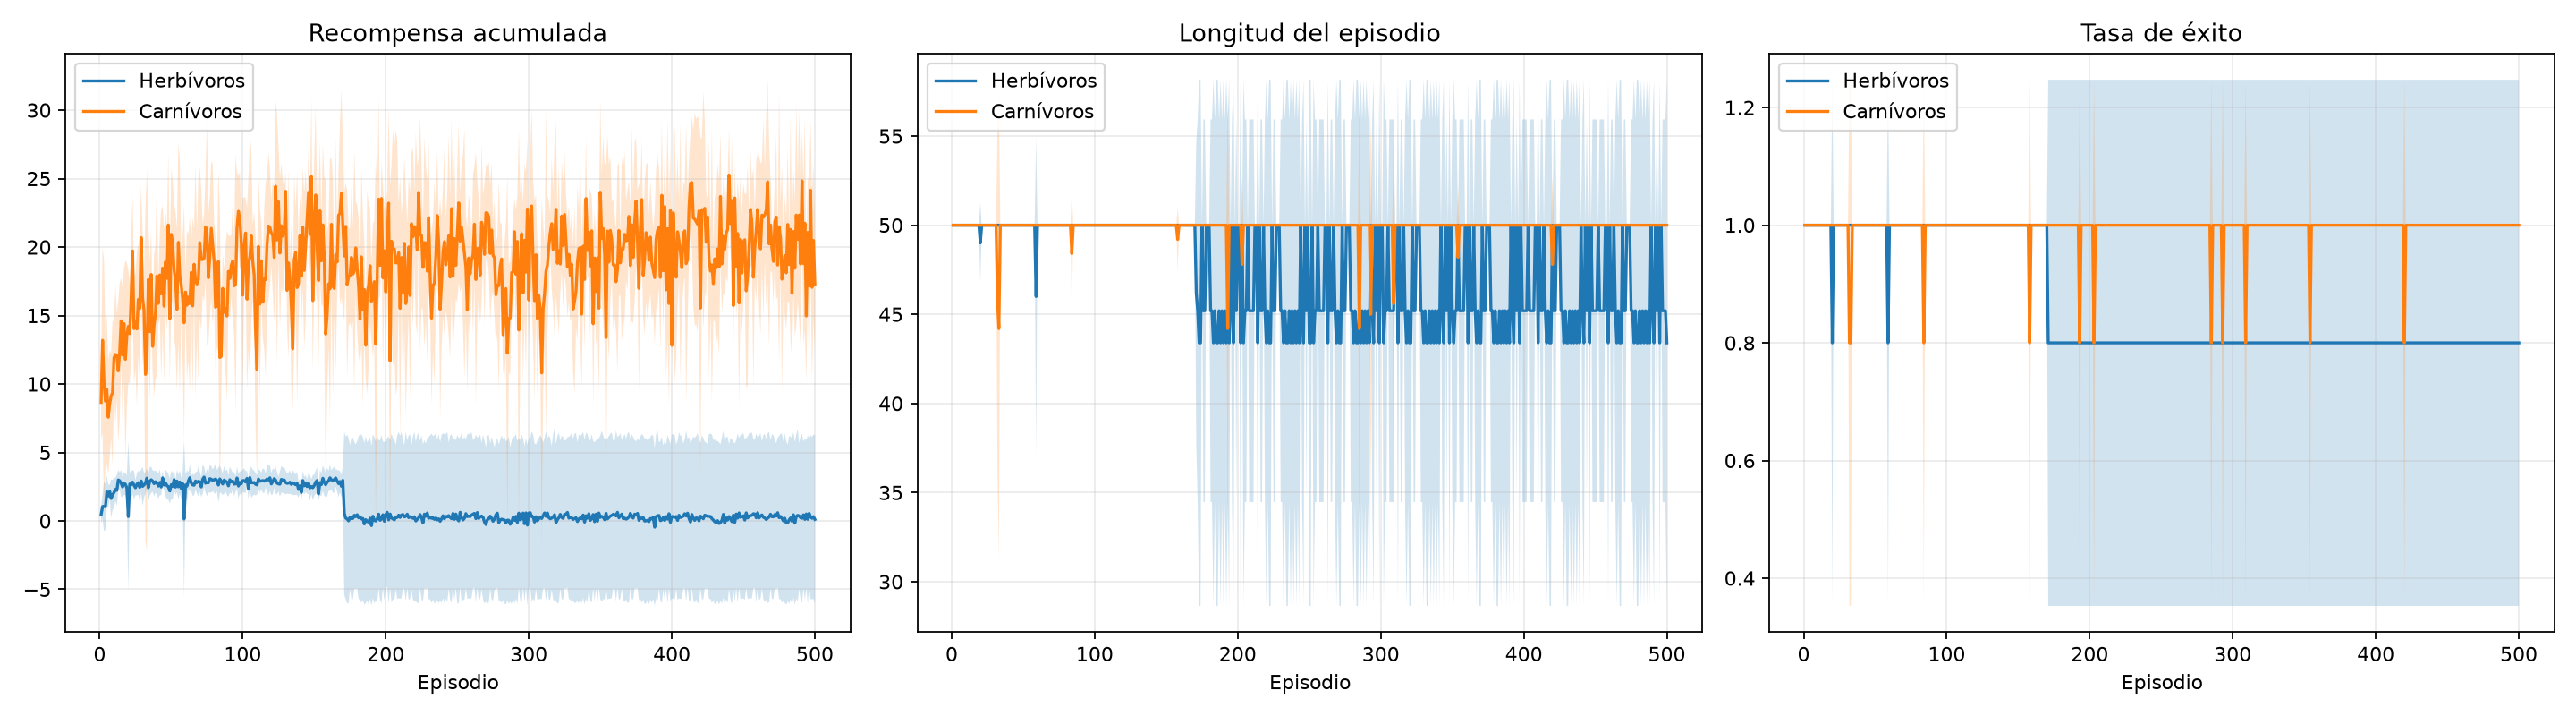
\includegraphics[width=\columnwidth]{experiments/stage2/training_curves.png}
\caption{Curvas de entrenamiento con bandas de dispersión.}
\label{fig:curvas-entrenamiento}
\end{figure}

\begin{figure}[t]
\centering
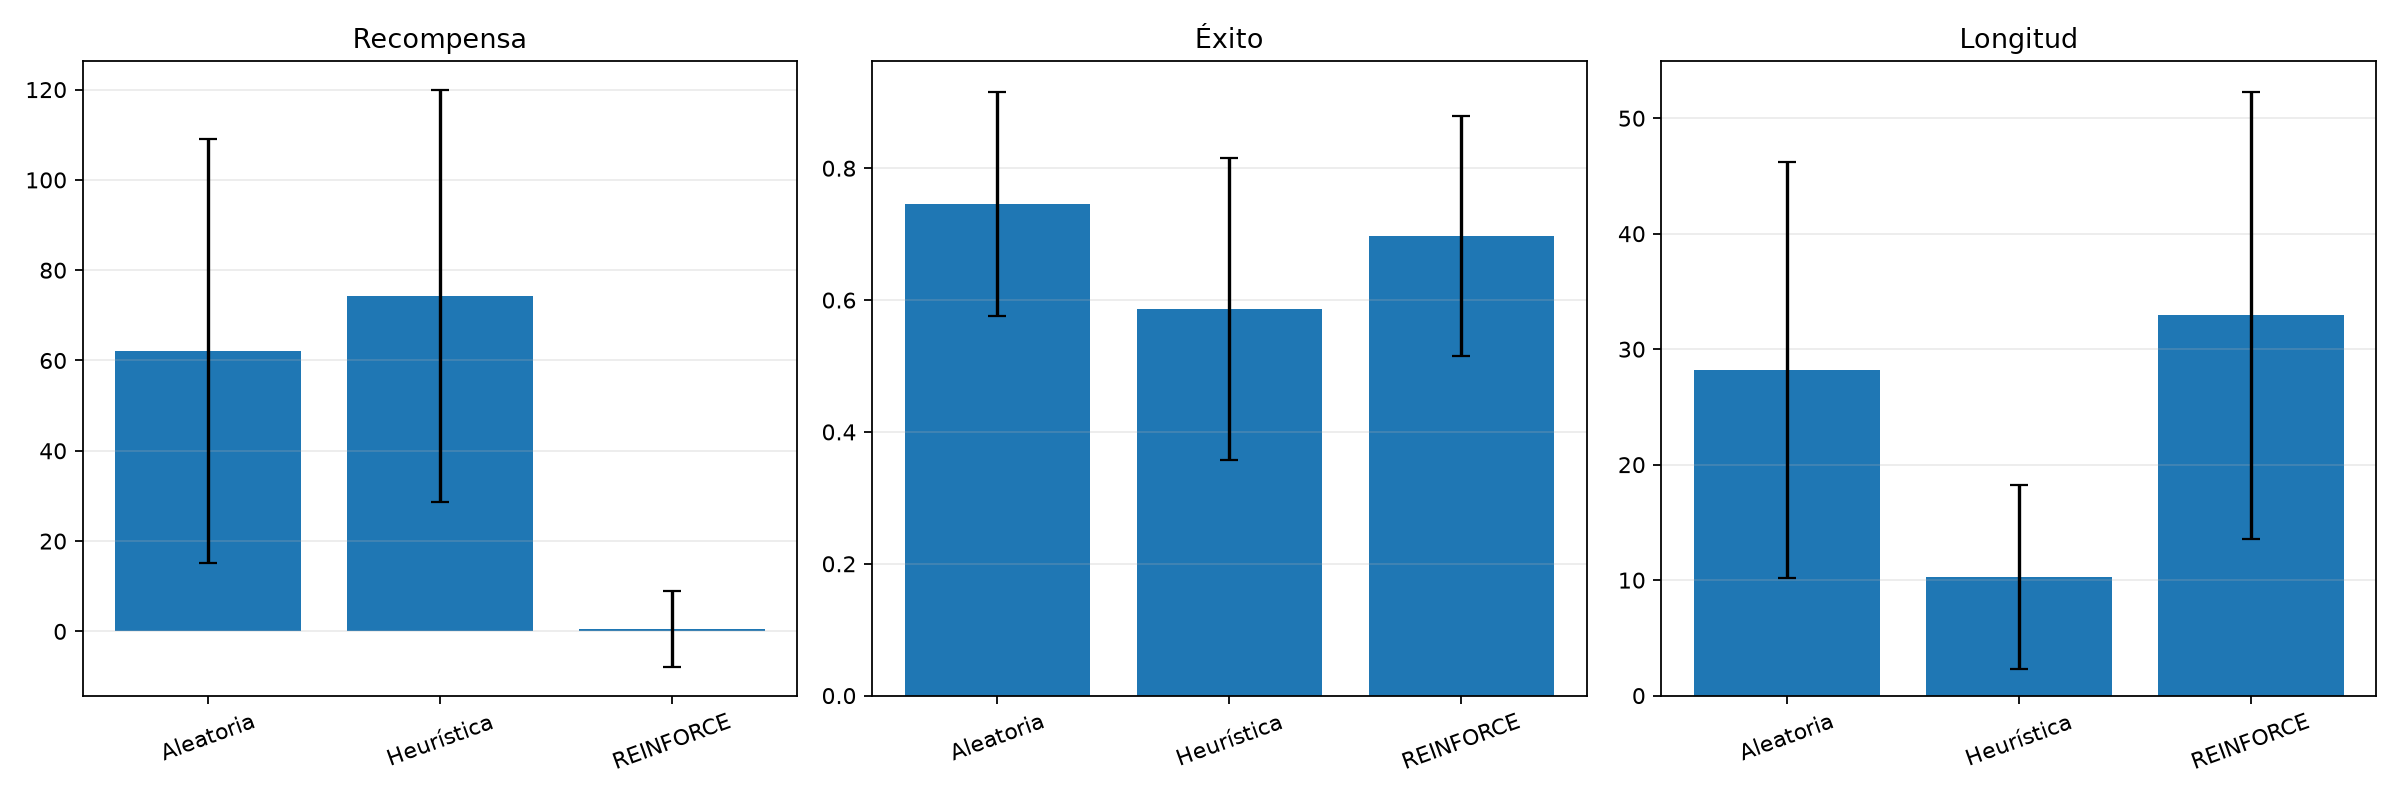
\includegraphics[width=\columnwidth]{experiments/stage2/evaluation_comparison.png}
\caption{Comparación de las políticas principales.}
\label{fig:comparacion-politicas}
\end{figure}

\subsection{Análisis de sensibilidad}

La Tabla~\ref{tab:sensibilidad} presenta el módulo adicional. $0.005$ obtiene
el mayor fitness y éxito promedio, además de la menor dispersión en longitud.
$0.010$ y $0.020$ producen los mismos resultados de evaluación por semilla,
aunque sus checkpoints tienen pesos distintos. Esto es compatible con la
evaluación determinista sin exploración: ambos modelos pueden seleccionar las
mismas acciones discretas de mayor logit.

\begin{table}[t]
\centering
\caption{Sensibilidad a la tasa de aprendizaje: media $\pm$ desviación estándar entre tres semillas.}
\label{tab:sensibilidad}
\begin{tabular}{lrrrr}
\toprule
$\alpha$ & Fitness & Recompensa & Éxito & Longitud \\
\midrule
0.005 & $0.5184\pm0.0882$ & $-1.5560\pm3.4705$ &
$0.7133\pm0.1514$ & $38.37\pm2.76$ \\
0.010 & $0.4766\pm0.0599$ & $-1.4470\pm2.4047$ &
$0.6343\pm0.1160$ & $26.73\pm16.08$ \\
0.020 & $0.4766\pm0.0599$ & $-1.4470\pm2.4047$ &
$0.6343\pm0.1160$ & $26.73\pm16.08$ \\
\bottomrule
\end{tabular}
\end{table}

\begin{figure}[t]
\centering
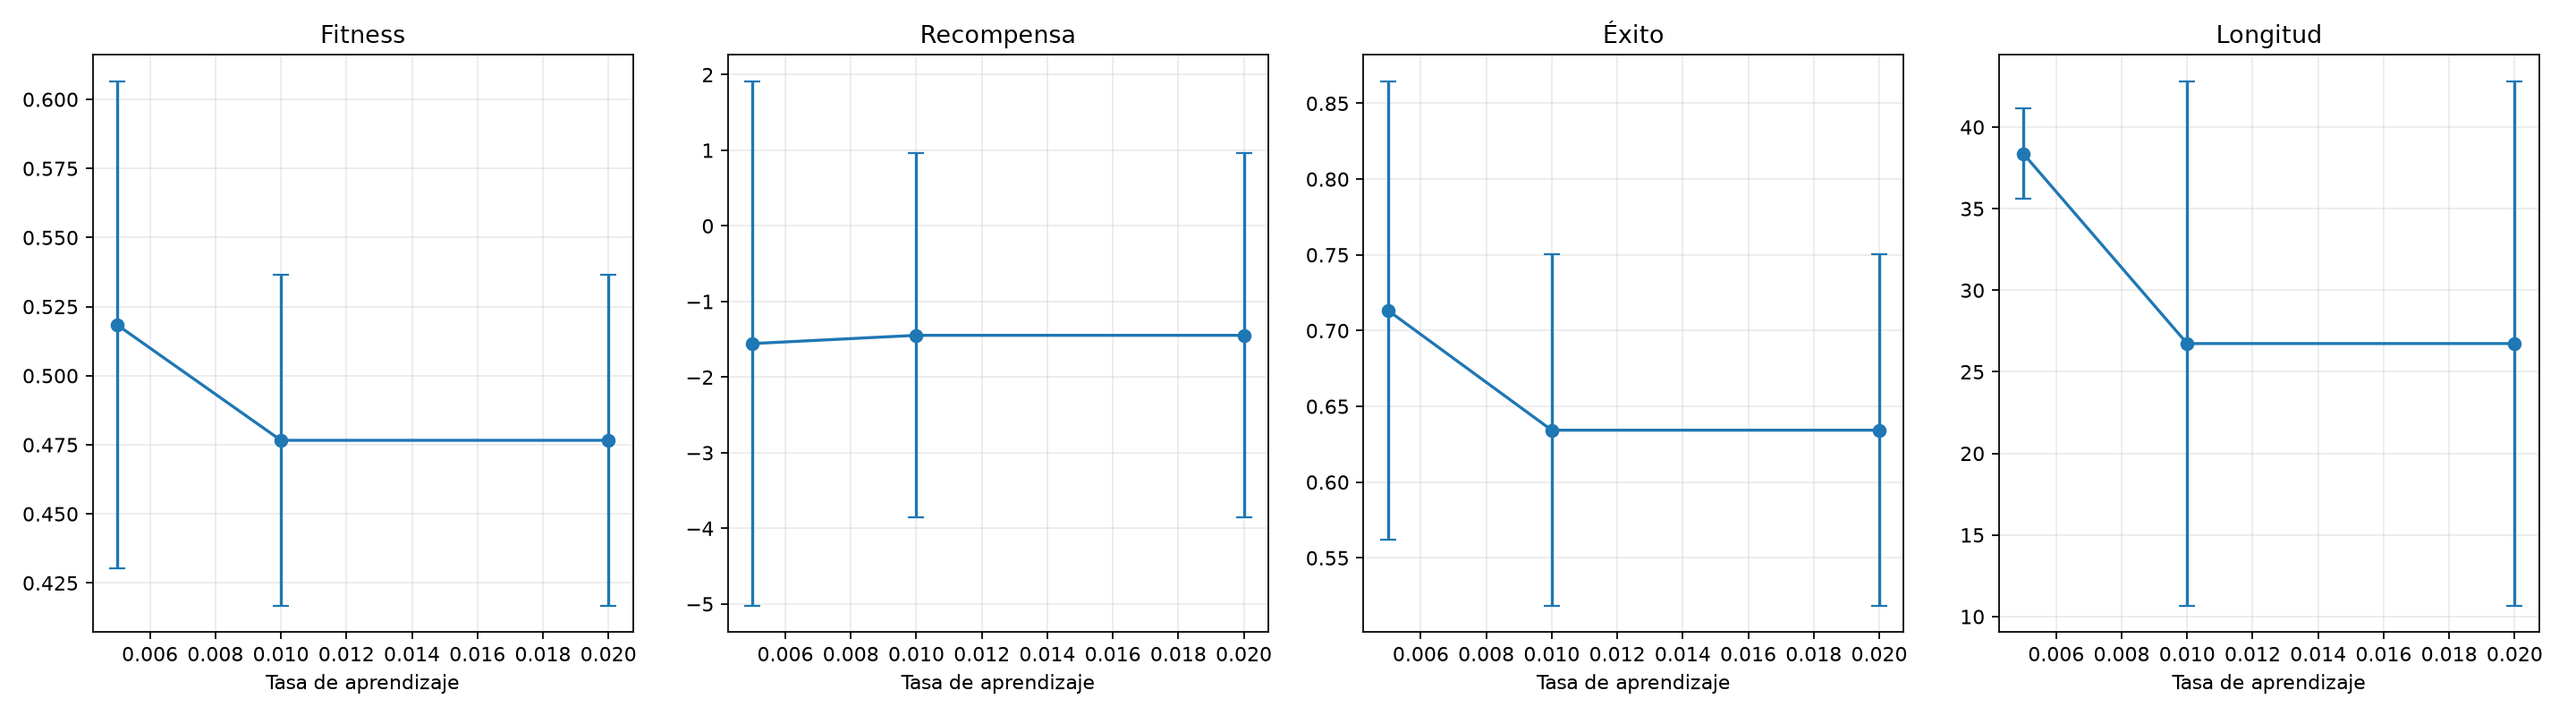
\includegraphics[width=\columnwidth]{experiments/sensitivity/sensitivity_comparison.png}
\caption{Sensibilidad de las métricas a la tasa de aprendizaje.}
\label{fig:sensibilidad}
\end{figure}

\subsection{Análisis cualitativo}

El herbívoro alterna desplazamiento y consumo; el descanso resulta útil con
energía baja, pero es penalizado cuando la energía es suficiente. El carnívoro
busca coincidencias espaciales para ejecutar \texttt{HUNT}, por lo que la
cacería depende de compartir la misma celda. La reproducción requiere dos
individuos elegibles en la misma celda; cuando la energía cae o no existe una
pareja cercana, no se producen nacimientos. La exploración se usa durante el
entrenamiento y se desactiva durante la evaluación.

% ---------------------------------------------------------
% REFERENCIAS
% ---------------------------------------------------------

\begin{thebibliography}{99}

\bibitem{Paper1}
S. Sokoloski \textit{et al.}, ``A computational approach to visual ecology with deep reinforcement learning,'' \textit{arXiv}, 2024. [Online]. Disponible: \url{https://arxiv.org/abs/2402.05266}

\bibitem{Paper2}
C. Strannegård \textit{et al.}, ``Agent-based ecosystem modeling with deep reinforcement learning,'' \textit{ScienceDirect}, 2026. [Online]. Disponible: \url{https://www.sciencedirect.com/science/article/pii/S1574954126002256}

\bibitem{Paper3}
M. Lapeyrolerie \textit{et al.}, ``Deep reinforcement learning for conservation decisions,'' \textit{British Ecological Society}, 2022. [Online]. Disponible: \url{https://besjournals.onlinelibrary.wiley.com/doi/epdf/10.1111/2041-210X.13954}

\bibitem{Paper4}
Y. Fonseca \textit{et al.}, ``World Models Unlock Optimal Foraging Strategies in Reinforcement Learning Agents,'' \textit{arXiv}, 2025. [Online]. Disponible: \url{https://arxiv.org/abs/2512.12548}

\bibitem{Paper5}
J. Brea \textit{et al.}, ``Computational models of episodic-like memory in food-caching birds,'' \textit{Nature Communications}, 2023. [Online]. Disponible: \url{https://www.nature.com/articles/s41467-023-38570-x}

\bibitem{Paper6}
S. Coleman \textit{et al.}, ``A neural network model of foraging decisions made under predation risk,'' \textit{Springer Nature Link}, 2005. [Online]. Disponible: \url{https://link.springer.com/article/10.3758/CABN.5.4.434}

\bibitem{Paper7}
R. Urbaniak \textit{et al.}, ``Linking cognitive strategy, neural mechanism, and movement statistics in group foraging behaviors,'' \textit{Scientific Reports}, 2024. [Online]. Disponible: \url{https://www.nature.com/articles/s41598-024-71931-0}

\bibitem{Paper8}
A. Zia \textit{et al.}, ``A review on vision-centric coarse to fine-grained animal action recognition,'' \textit{Springer Nature Link}, 2026. [Online]. Disponible: \url{https://link.springer.com/article/10.1007/s10462-026-11526-5}

\bibitem{Survey1}
D. DeAngelis \& S. Diaz, ``Decision-Making in Agent-Based Modeling: A Current Review and Future Prospectus,'' \textit{Frontiers in Ecology and Evolution}, 2019. [Online]. Disponible: \url{https://www.frontiersin.org/journals/ecology-and-evolution/articles/10.3389/fevo.2018.00237/full}

\bibitem{Paper9}
G. Zheng \textit{et al.}, ``A brief review of evolutionary game dynamics in the reinforcement learning paradigm,'' \textit{arXiv}, 2026. [Online]. Disponible: \url{https://arxiv.org/abs/2602.04150}

\bibitem{Paper10}
J. Willoughby \textit{et al.}, ``Using AI enhanced agent-based models to support management of wild populations,'' \textit{Springer Nature Link}, 2025. [Online]. Disponible: \url{https://link.springer.com/article/10.1007/s10980-025-02149-2}

\bibitem{Paper11}
A. Caftory \textit{et al.}, ``Why Study Emergent Behavior When You Can Regulate It? Aligning Multi-Agent Systems with Reward Prediction,'' \textit{arXiv}, 2026. [Online]. Disponible: \url{https://arxiv.org/pdf/2608.07280v1}

\bibitem{Paper12}
A. Yamaguchi, ``Emergent Coordination and Phase Structure in Independent Multi-Agent Reinforcement Learning,'' \textit{arXiv}, 2025. [Online]. Disponible: \url{https://arxiv.org/pdf/2511.23315v1}

\bibitem{Paper13}
Z. Kilpatrick \textit{et al.}, ``Resource depletion accelerates rate learning but not composition learning in patch foraging,'' \textit{arXiv}, 2026. [Online]. Disponible: \url{https://arxiv.org/html/2607.29476v1}

\bibitem{Paper14}
R. Pihlakas \textit{et al.}, ``From homeostasis to resource sharing: Biologically and economically aligned multi-objective multi-agent gridworld-based AI safety benchmarks,'' \textit{arXiv}, 2025. [Online]. Disponible: \url{https://arxiv.org/html/2410.00081v5}

\bibitem{Survey2}
M. Zerrouk \textit{et al.}, ``Machine and Deep Learning for Wetland Mapping and Bird-Habitat Monitoring: A Systematic Review of Remote-Sensing Applications,'' \textit{MDPI}, 2025. [Online]. Disponible: \url{https://www.mdpi.com/2072-4292/17/21/3605}

\bibitem{Paper15}
S. Barton \textit{et al.}, ``Measuring collaborative emergent behavior in multiagent reinforcement learning,'' \textit{arXiv}, 2018. [Online]. Disponible: \url{https://arxiv.org/pdf/1807.08663}

\bibitem{Paper16}
S. Xu and Z. Dang, ``Emergent Behaviors in Multiagent Pursuit-Evasion Games Within a Bounded 2D Grid World,'' \textit{National Library of Medicine - PMC Biomedical Research}, 2025. [Online]. Disponible: \url{https://pmc.ncbi.nlm.nih.gov/articles/PMC12340135/}

\bibitem{Paper17}
M. Brambati \textit{et al.}, ``Learning to Flock in Open Space by Avoiding Collisions and Staying Together,'' \textit{arXiv}, 2026. [Online]. Disponible: \url{https://arxiv.org/pdf/2506.15587}

\bibitem{Paper18}
C. Hahn \textit{et al.}, ``Foraging Swarms Using Multi-Agent Reinforcement Learning,'' \textit{MIT Press Direct}, 2020. [Online]. Disponible: \url{https://direct.mit.edu/isal/article/doi/10.1162/isal_a_00267/98496}

\bibitem{Paper19}
M. Kölle \textit{et al.}, ``Aquarium: A Comprehensive Framework for Exploring Predator-Prey Dynamics through Multi-Agent Reinforcement Learning Algorithms,'' \textit{arXiv}, 2024. [Online]. Disponible: \url{https://arxiv.org/abs/2401.07056}

\bibitem{Paper20}
A. López-Incera \textit{et al.}, ``Development of Swarm Behavior in Artificial Learning Agents That Adapt to Different Foraging Environment,'' \textit{National Library of Medicine - PMC Biomedical Research}, 2020. [Online]. Disponible: \url{https://www.ncbi.nlm.nih.gov/pmc/articles/PMC7748156/}

\bibitem{Survey3}
S. Gronauer \& K. Diepold, ``Multi-Agent Deep Reinforcement Learning: A Survey,'' \textit{Springer Nature Link - Artificial Intelligence Review}, 2021. [Online]. Disponible: \url{https://link.springer.com/article/10.1007/s10462-021-09996-w}

\end{thebibliography}

\end{document}